% Options for packages loaded elsewhere
\PassOptionsToPackage{unicode}{hyperref}
\PassOptionsToPackage{hyphens}{url}
%
\documentclass[
  letterpaper,
]{book}

\usepackage{amsmath,amssymb}
\usepackage{lmodern}
\usepackage{iftex}
\ifPDFTeX
  \usepackage[T1]{fontenc}
  \usepackage[utf8]{inputenc}
  \usepackage{textcomp} % provide euro and other symbols
\else % if luatex or xetex
  \usepackage{unicode-math}
  \defaultfontfeatures{Scale=MatchLowercase}
  \defaultfontfeatures[\rmfamily]{Ligatures=TeX,Scale=1}
\fi
% Use upquote if available, for straight quotes in verbatim environments
\IfFileExists{upquote.sty}{\usepackage{upquote}}{}
\IfFileExists{microtype.sty}{% use microtype if available
  \usepackage[]{microtype}
  \UseMicrotypeSet[protrusion]{basicmath} % disable protrusion for tt fonts
}{}
\makeatletter
\@ifundefined{KOMAClassName}{% if non-KOMA class
  \IfFileExists{parskip.sty}{%
    \usepackage{parskip}
  }{% else
    \setlength{\parindent}{0pt}
    \setlength{\parskip}{6pt plus 2pt minus 1pt}}
}{% if KOMA class
  \KOMAoptions{parskip=half}}
\makeatother
\usepackage{xcolor}
\setlength{\emergencystretch}{3em} % prevent overfull lines
\setcounter{secnumdepth}{5}
% Make \paragraph and \subparagraph free-standing
\ifx\paragraph\undefined\else
  \let\oldparagraph\paragraph
  \renewcommand{\paragraph}[1]{\oldparagraph{#1}\mbox{}}
\fi
\ifx\subparagraph\undefined\else
  \let\oldsubparagraph\subparagraph
  \renewcommand{\subparagraph}[1]{\oldsubparagraph{#1}\mbox{}}
\fi

\usepackage{color}
\usepackage{fancyvrb}
\newcommand{\VerbBar}{|}
\newcommand{\VERB}{\Verb[commandchars=\\\{\}]}
\DefineVerbatimEnvironment{Highlighting}{Verbatim}{commandchars=\\\{\}}
% Add ',fontsize=\small' for more characters per line
\usepackage{framed}
\definecolor{shadecolor}{RGB}{241,243,245}
\newenvironment{Shaded}{\begin{snugshade}}{\end{snugshade}}
\newcommand{\AlertTok}[1]{\textcolor[rgb]{0.68,0.00,0.00}{#1}}
\newcommand{\AnnotationTok}[1]{\textcolor[rgb]{0.37,0.37,0.37}{#1}}
\newcommand{\AttributeTok}[1]{\textcolor[rgb]{0.40,0.45,0.13}{#1}}
\newcommand{\BaseNTok}[1]{\textcolor[rgb]{0.68,0.00,0.00}{#1}}
\newcommand{\BuiltInTok}[1]{\textcolor[rgb]{0.00,0.23,0.31}{#1}}
\newcommand{\CharTok}[1]{\textcolor[rgb]{0.13,0.47,0.30}{#1}}
\newcommand{\CommentTok}[1]{\textcolor[rgb]{0.37,0.37,0.37}{#1}}
\newcommand{\CommentVarTok}[1]{\textcolor[rgb]{0.37,0.37,0.37}{\textit{#1}}}
\newcommand{\ConstantTok}[1]{\textcolor[rgb]{0.56,0.35,0.01}{#1}}
\newcommand{\ControlFlowTok}[1]{\textcolor[rgb]{0.00,0.23,0.31}{#1}}
\newcommand{\DataTypeTok}[1]{\textcolor[rgb]{0.68,0.00,0.00}{#1}}
\newcommand{\DecValTok}[1]{\textcolor[rgb]{0.68,0.00,0.00}{#1}}
\newcommand{\DocumentationTok}[1]{\textcolor[rgb]{0.37,0.37,0.37}{\textit{#1}}}
\newcommand{\ErrorTok}[1]{\textcolor[rgb]{0.68,0.00,0.00}{#1}}
\newcommand{\ExtensionTok}[1]{\textcolor[rgb]{0.00,0.23,0.31}{#1}}
\newcommand{\FloatTok}[1]{\textcolor[rgb]{0.68,0.00,0.00}{#1}}
\newcommand{\FunctionTok}[1]{\textcolor[rgb]{0.28,0.35,0.67}{#1}}
\newcommand{\ImportTok}[1]{\textcolor[rgb]{0.00,0.46,0.62}{#1}}
\newcommand{\InformationTok}[1]{\textcolor[rgb]{0.37,0.37,0.37}{#1}}
\newcommand{\KeywordTok}[1]{\textcolor[rgb]{0.00,0.23,0.31}{#1}}
\newcommand{\NormalTok}[1]{\textcolor[rgb]{0.00,0.23,0.31}{#1}}
\newcommand{\OperatorTok}[1]{\textcolor[rgb]{0.37,0.37,0.37}{#1}}
\newcommand{\OtherTok}[1]{\textcolor[rgb]{0.00,0.23,0.31}{#1}}
\newcommand{\PreprocessorTok}[1]{\textcolor[rgb]{0.68,0.00,0.00}{#1}}
\newcommand{\RegionMarkerTok}[1]{\textcolor[rgb]{0.00,0.23,0.31}{#1}}
\newcommand{\SpecialCharTok}[1]{\textcolor[rgb]{0.37,0.37,0.37}{#1}}
\newcommand{\SpecialStringTok}[1]{\textcolor[rgb]{0.13,0.47,0.30}{#1}}
\newcommand{\StringTok}[1]{\textcolor[rgb]{0.13,0.47,0.30}{#1}}
\newcommand{\VariableTok}[1]{\textcolor[rgb]{0.07,0.07,0.07}{#1}}
\newcommand{\VerbatimStringTok}[1]{\textcolor[rgb]{0.13,0.47,0.30}{#1}}
\newcommand{\WarningTok}[1]{\textcolor[rgb]{0.37,0.37,0.37}{\textit{#1}}}

\providecommand{\tightlist}{%
  \setlength{\itemsep}{0pt}\setlength{\parskip}{0pt}}\usepackage{longtable,booktabs,array}
\usepackage{calc} % for calculating minipage widths
% Correct order of tables after \paragraph or \subparagraph
\usepackage{etoolbox}
\makeatletter
\patchcmd\longtable{\par}{\if@noskipsec\mbox{}\fi\par}{}{}
\makeatother
% Allow footnotes in longtable head/foot
\IfFileExists{footnotehyper.sty}{\usepackage{footnotehyper}}{\usepackage{footnote}}
\makesavenoteenv{longtable}
\usepackage{graphicx}
\makeatletter
\def\maxwidth{\ifdim\Gin@nat@width>\linewidth\linewidth\else\Gin@nat@width\fi}
\def\maxheight{\ifdim\Gin@nat@height>\textheight\textheight\else\Gin@nat@height\fi}
\makeatother
% Scale images if necessary, so that they will not overflow the page
% margins by default, and it is still possible to overwrite the defaults
% using explicit options in \includegraphics[width, height, ...]{}
\setkeys{Gin}{width=\maxwidth,height=\maxheight,keepaspectratio}
% Set default figure placement to htbp
\makeatletter
\def\fps@figure{htbp}
\makeatother
\newlength{\cslhangindent}
\setlength{\cslhangindent}{1.5em}
\newlength{\csllabelwidth}
\setlength{\csllabelwidth}{3em}
\newlength{\cslentryspacingunit} % times entry-spacing
\setlength{\cslentryspacingunit}{\parskip}
\newenvironment{CSLReferences}[2] % #1 hanging-ident, #2 entry spacing
 {% don't indent paragraphs
  \setlength{\parindent}{0pt}
  % turn on hanging indent if param 1 is 1
  \ifodd #1
  \let\oldpar\par
  \def\par{\hangindent=\cslhangindent\oldpar}
  \fi
  % set entry spacing
  \setlength{\parskip}{#2\cslentryspacingunit}
 }%
 {}
\usepackage{calc}
\newcommand{\CSLBlock}[1]{#1\hfill\break}
\newcommand{\CSLLeftMargin}[1]{\parbox[t]{\csllabelwidth}{#1}}
\newcommand{\CSLRightInline}[1]{\parbox[t]{\linewidth - \csllabelwidth}{#1}\break}
\newcommand{\CSLIndent}[1]{\hspace{\cslhangindent}#1}

\makeatletter
\makeatother
\makeatletter
\@ifpackageloaded{bookmark}{}{\usepackage{bookmark}}
\makeatother
\makeatletter
\@ifpackageloaded{caption}{}{\usepackage{caption}}
\AtBeginDocument{%
\ifdefined\contentsname
  \renewcommand*\contentsname{Table of contents}
\else
  \newcommand\contentsname{Table of contents}
\fi
\ifdefined\listfigurename
  \renewcommand*\listfigurename{List of Figures}
\else
  \newcommand\listfigurename{List of Figures}
\fi
\ifdefined\listtablename
  \renewcommand*\listtablename{List of Tables}
\else
  \newcommand\listtablename{List of Tables}
\fi
\ifdefined\figurename
  \renewcommand*\figurename{Figure}
\else
  \newcommand\figurename{Figure}
\fi
\ifdefined\tablename
  \renewcommand*\tablename{Table}
\else
  \newcommand\tablename{Table}
\fi
}
\@ifpackageloaded{float}{}{\usepackage{float}}
\floatstyle{ruled}
\@ifundefined{c@chapter}{\newfloat{codelisting}{h}{lop}}{\newfloat{codelisting}{h}{lop}[chapter]}
\floatname{codelisting}{Listing}
\newcommand*\listoflistings{\listof{codelisting}{List of Listings}}
\makeatother
\makeatletter
\@ifpackageloaded{caption}{}{\usepackage{caption}}
\@ifpackageloaded{subcaption}{}{\usepackage{subcaption}}
\makeatother
\makeatletter
\@ifpackageloaded{tcolorbox}{}{\usepackage[many]{tcolorbox}}
\makeatother
\makeatletter
\@ifundefined{shadecolor}{\definecolor{shadecolor}{rgb}{.97, .97, .97}}
\makeatother
\makeatletter
\makeatother
\ifLuaTeX
  \usepackage{selnolig}  % disable illegal ligatures
\fi
\IfFileExists{bookmark.sty}{\usepackage{bookmark}}{\usepackage{hyperref}}
\IfFileExists{xurl.sty}{\usepackage{xurl}}{} % add URL line breaks if available
\urlstyle{same} % disable monospaced font for URLs
\hypersetup{
  pdftitle={Quantiles},
  pdfauthor={andrew p.~blake},
  hidelinks,
  pdfcreator={LaTeX via pandoc}}

\title{Quantiles}
\author{andrew p.~blake}
\date{6/5/24}

\begin{document}
\frontmatter
\maketitle
\ifdefined\Shaded\renewenvironment{Shaded}{\begin{tcolorbox}[enhanced, breakable, boxrule=0pt, borderline west={3pt}{0pt}{shadecolor}, interior hidden, frame hidden, sharp corners]}{\end{tcolorbox}}\fi

\renewcommand*\contentsname{Table of contents}
{
\setcounter{tocdepth}{2}
\tableofcontents
}
\mainmatter
\bookmarksetup{startatroot}

\hypertarget{preface}{%
\chapter*{Preface}\label{preface}}
\addcontentsline{toc}{chapter}{Preface}

\markboth{Preface}{Preface}

This book is the result of an initiative that the Bank of England began
in the early 1990s. This was a different world with a burgeoning new
world order, as the Iron Curtain crumbled and the European experiment
gathered momentum.

Placeholders abound.

\emph{Disclaimer: The Bank of England does not accept any liability for
misleading or inaccurate information or omissions in the information
provided. The subject matter reflects the views of the individual
presenter and not the wider Bank of England or its Policy Committees.}

\bookmarksetup{startatroot}

\hypertarget{introduction}{%
\chapter{Introduction}\label{introduction}}

This is a book created from markdown and executable code.

See Blake and Mumtaz (2017).

\begin{center}\rule{0.5\linewidth}{0.5pt}\end{center}

\hypertarget{reading-is-good-for-you}{%
\section{Reading is good for you}\label{reading-is-good-for-you}}

For me, the best (although slightly dated) text is Hastie, Tibshirani,
and Friedman (2009)
\href{https://web.stanford.edu/~hastie/ElemStatLearn/}{The Elements of
Statistical Learning} and the best source for the mathematics, with an
easy-reading version by some of the same authors James et al. (2021)
\href{https://www.statlearning.com/}{Introduction to Statistical
Learning}.

I also rather like Boehmke and Greenwell (2019)
\href{https://bradleyboehmke.github.io/HOML/}{Hands-On Machine Learning
with R} which is something of a cookbook rather than a technical manual
but with wide scope. Taddy (2019) is more elementary.

On text, just read Silge and Robinson (2017)
\href{https://www.tidytextmining.com/}{Text Mining with R: A Tidy
Approach} and then Hvitfeldt and Silge (2021)
\href{https://smltar.com/}{Supervised Machine Learning for Text Analysis
in R}. That's it.

Two books I would solidly recommend to make us all into better
statisticians and not just econometricians are Gelman, Hill, and Vehtari
(2019) \href{http://www.stat.columbia.edu/~gelman/regression}{Regression
and Other Stories}, and McElreath (2020)
\href{https://github.com/rmcelreath/rethinking}{Statistical Rethinking}.

\bookmarksetup{startatroot}

\hypertarget{non-econometric-methods-for-econometricians}{%
\chapter{Non-econometric methods for
econometricians}\label{non-econometric-methods-for-econometricians}}

\hypertarget{selected-ml-and-dataviz-techniques-using-r}{%
\section{Selected ML and Dataviz techniques using
R}\label{selected-ml-and-dataviz-techniques-using-r}}

Econometricians are used to handling data, performing analysis and
reporting results. But somewhere along the line data became big and
unstructured, analysis was now machines learning about something and
outputs became visualisations.

This online seminar takes some big(ish) datasets, sets the machines on
them and draws some great graphs. If you ever wondered what use a tree
was for forecasting or why everything is a network (including neural
ones), or wanted to draw a map with your house in it, or to understand a
document without the bother of reading it (or a few other things
besides) then you might find something to interest you. All done in R.

Specifically, this seminar is designed to introduce some of the key
methods used outside of econometrics that econometricians will find very
useful in their work in a central bank. This includes some important
machine learning techniques as a gateway to others, particularly
tree-based methods and neural networks, as well as text processing and
map making. All the way through there is an emphasis on the network
properties of many of these techniques. We make extensive use of the
\texttt{tidyverse}, including \texttt{ggplot2} and \texttt{tidytext},
and a number of statistics, machine learning, geographical data and
other packages.

The framework for each day is the following:

\begin{itemize}
\tightlist
\item
  Each day is divided into two two-hour sessions starting at 10.30 am
  and 2.00 pm GMT.
\item
  The first hour of each will be an online presentation covering a
  particular topic (or topics) with a look at both techniques and code.
\item
  After a quick break the second hour will be largely devoted to the
  code itself or resources to understand how to code the material.
\end{itemize}

We may run polls during the event to prioritize the topics covered in
the webinars as it is not expected that everyone will be able to try out
everything.

\hypertarget{the-code}{%
\subsection{The code}\label{the-code}}

All code and some of the data will be made available through the Juno
portal. For each presentation the .Rmd (R markdown) file is supplied
that creates the presentation, an HTML file of the presentation for you
to step through which can be re-created from the .Rmd file, and a
further .R file of the code that we use. Some additional code and data
is included, including links to a number of videos that cover some
additional aspects both in this file and in the presentations.

Some data will need to be downloaded from original other sites if all
the examples are to be followed. All code is additionally available at
\url{https://github.com/andrewpeterblake/R2020} or
\url{https://github.com/andrewpeterblake/R2021} or through the QR codes
below.

\begin{figure}

{\centering 
\includegraphics[width=0.25\textwidth,height=\textheight]{./R2021_files/figure-pdf/unnamed-chunk-1-1.pdf}

}

\caption{GitHub: 2020 (grey, left), 2021 (pink, right)}

\end{figure}

\begin{figure}

{\centering 
\includegraphics[width=0.25\textwidth,height=\textheight]{./R2021_files/figure-pdf/unnamed-chunk-1-2.pdf}

}

\caption{GitHub: 2020 (grey, left), 2021 (pink, right)}

\end{figure}

\begin{center}\rule{0.5\linewidth}{0.5pt}\end{center}

\hypertarget{how-to-ensure-rstudio-finds-the-code}{%
\section{HOW TO ENSURE RSTUDIO FINDS THE
CODE}\label{how-to-ensure-rstudio-finds-the-code}}

To use the code, in particular so that R Studio finds the data files
etc, create a directory for each topic, (e.g.~Trees, ANN etc) and copy
the contents from the zip file or GitHub. Then create a new project in R
Studio that uses that directory as its home directory, using ``File/New
Project'' in the drop down menu. Opening files within a project sets the
home directory to that directory, so everything (including the
sub-directories) can be found.

\begin{center}\rule{0.5\linewidth}{0.5pt}\end{center}

\hypertarget{typical-program-structure}{%
\section{Typical program structure}\label{typical-program-structure}}

\hypertarget{day-1-trees-and-maps}{%
\subsection{Day 1: Trees and maps}\label{day-1-trees-and-maps}}

\hypertarget{trees}{%
\subsubsection{Trees}\label{trees}}

\begin{itemize}
\tightlist
\item
  Classification and regression trees
\item
  Econometrics strikes back: Bootstrap/bagging and Boosting/Model
  selection
\item
  Random forests
\item
  Visualising decision trees
\item
  Use example: House prices
\end{itemize}

The presentations for this are \texttt{Trees.html} and
\texttt{LondonHP.html}; The two programs \texttt{TreeCancer.R} and
\texttt{TreeNW.R} are the use examples.

\hypertarget{maps}{%
\subsubsection{Maps}\label{maps}}

\begin{itemize}
\tightlist
\item
  How to draw a map in R
\item
  A guide to some resources
\item
  Choropleths
\item
  Use examples: Climate change, regional data, postcode wrangling
\end{itemize}

The presentation for this is \texttt{MapAER.html} (see also
\texttt{Weatherpretty.html}); The program \texttt{MapAERcode.R} is the
main map drawing code, I've included \texttt{ZAF.R} as as short simple
way and source for two countries, and the directory \texttt{Trendz}
contains the program (\texttt{app.R}) and data for the weather example.

\begin{figure}

\hfill{} 
\includegraphics[width=0.5\textwidth,height=\textheight]{./R2021_files/figure-pdf/unnamed-chunk-2-1.pdf}

\end{figure}

I've included an additional video (red QR code) for more about Shiny.
This uses unemployment data from the
\href{https://www.philadelphiafed.org/surveys-and-data/real-time-data-research/survey-of-professional-forecasters}{Survey
of Professional Forecasters}. The code we look at is for climate change
data \href{https://climateknowledgeportal.worldbank.org/}{World Bank
data}.

A comprehensive treatment of maps is Lovelace, Nowosad, and Muenchow
(2019) \emph{Geocomputation in R}, but it is quite a lot to assimilate
all at once.

\begin{center}\rule{0.5\linewidth}{0.5pt}\end{center}

\hypertarget{day-2-networks}{%
\subsection{Day 2: Networks}\label{day-2-networks}}

\hypertarget{neural-networks}{%
\subsubsection{Neural networks}\label{neural-networks}}

\begin{itemize}
\tightlist
\item
  What is an ANN? Deep learning?
\item
  Function approximation via a network
\item
  Data: fit, validate, test
\item
  Network architecture
\item
  Use examples: House prices revisited
\end{itemize}

The presentation for this is \texttt{IntroANN.html}; The program
\texttt{ANN.R} replicates the ANN estimation. The data used is the same
as for Day 1.

\hypertarget{networks-real-ones}{%
\subsubsection{Networks (real ones)}\label{networks-real-ones}}

\begin{itemize}
\tightlist
\item
  DAGs and ANNs as network graphs
\item
  Incidence matrices
\item
  Measuring connectivity: Degree and betweenness
\item
  Plotting with \texttt{igraph}
\item
  Use examples: Industry inter-relationships
\end{itemize}

\begin{figure}

\hfill{} 
\includegraphics[width=0.25\textwidth,height=\textheight]{./R2021_files/figure-pdf/unnamed-chunk-3-1.pdf}

\end{figure}

\begin{figure}

\hfill{} 
\includegraphics[width=0.25\textwidth,height=\textheight]{./R2021_files/figure-pdf/unnamed-chunk-3-2.pdf}

\end{figure}

The presentation used for the first part of this is \texttt{DAG.html}
and the program \texttt{Draw\_DAG\_ANN.R} draws the ANN examples from
Day 2 Session 1 as well as some of the DAG examples. The example is
modified from Cunningham (2021) \emph{Causal Inference: The Mixtape},
which is a great read with R code. The pdf \texttt{HandShake3.pdf} is
the source of the director network graphs, and \texttt{Graph101a.R} is a
subset of the analytical work on the corruption data set as described in
the post
\href{https://www.r-bloggers.com/2020/01/graph-theory-101-with-corruption-cases-in-spain/}{\emph{Graph
Theory 101}} (purple QR code), which is the work of
\href{https://codingclubuc3m.rbind.io/talk/2020-01-21/}{Marina Medina}
(blue QR code link to presentation site).

\begin{center}\rule{0.5\linewidth}{0.5pt}\end{center}

\hypertarget{day-3-text}{%
\subsection{Day 3: Text}\label{day-3-text}}

\hypertarget{text-modelling-a-tidytext-approach-session-1}{%
\subsubsection{Text modelling, a `tidytext' approach (Session
1)}\label{text-modelling-a-tidytext-approach-session-1}}

\begin{itemize}
\tightlist
\item
  Data cleaning
\item
  Sentiment
\item
  Topic modelling
\end{itemize}

\hypertarget{text-modelling-a-tidytext-approach-session-2}{%
\subsubsection{Text modelling, a `tidytext' approach (Session
2)}\label{text-modelling-a-tidytext-approach-session-2}}

\begin{itemize}
\tightlist
\item
  Parts-of-speech tagging
\item
  Text regression
\item
  Use examples: Central bank minutes, reports
\end{itemize}

\bookmarksetup{startatroot}

\hypertarget{quantile-regression-in-r}{%
\chapter{Quantile regression in R}\label{quantile-regression-in-r}}

This shows how to manipulate data from the SPF in R.

\begin{Shaded}
\begin{Highlighting}[]
\FunctionTok{library}\NormalTok{(readxl)}
\FunctionTok{library}\NormalTok{(xts)}
\FunctionTok{library}\NormalTok{(lubridate)}
\FunctionTok{library}\NormalTok{(tidyverse)}
\FunctionTok{library}\NormalTok{(quantmod)}
\FunctionTok{library}\NormalTok{(quantreg)}
\end{Highlighting}
\end{Shaded}

\hypertarget{getting-the-data}{%
\section{Getting the data}\label{getting-the-data}}

We download the data and save it locally.

\begin{Shaded}
\begin{Highlighting}[]
\NormalTok{h }\OtherTok{\textless{}{-}} \StringTok{"https://www.philadelphiafed.org/{-}/media/frbp/assets/surveys{-}and{-}data/survey{-}of{-}professional{-}forecasters/historical{-}data/"}
\NormalTok{f }\OtherTok{\textless{}{-}} \StringTok{"meanlevel.xlsx"}

\FunctionTok{download.file}\NormalTok{(}\FunctionTok{paste0}\NormalTok{(h, f), }\AttributeTok{destfile=}\NormalTok{f, }\AttributeTok{mode=}\StringTok{"wb"}\NormalTok{)}
\end{Highlighting}
\end{Shaded}

Retrieve the unemployment data for the average unemployment forecast.

\begin{Shaded}
\begin{Highlighting}[]
\NormalTok{UNEMP }\OtherTok{\textless{}{-}}\NormalTok{ f }\SpecialCharTok{\%\textgreater{}\%}
  \FunctionTok{read\_excel}\NormalTok{(}\AttributeTok{na=}\StringTok{"\#N/A"}\NormalTok{, }\AttributeTok{sheet=}\StringTok{"UNEMP"}\NormalTok{) }\SpecialCharTok{\%\textgreater{}\%} 
  \FunctionTok{mutate}\NormalTok{(}\AttributeTok{Date=}\FunctionTok{as.Date}\NormalTok{(}\FunctionTok{as.yearqtr}\NormalTok{(}\FunctionTok{paste}\NormalTok{(YEAR, QUARTER), }\AttributeTok{format=}\StringTok{"\%Y \%q"}\NormalTok{))) }

\NormalTok{Usel }\OtherTok{\textless{}{-}}\NormalTok{ UNEMP }\SpecialCharTok{\%\textgreater{}\%} 
  \FunctionTok{select}\NormalTok{(Date, UNEMP1, UNEMP3, UNEMP4, UNEMP5, UNEMP6) }\SpecialCharTok{\%\textgreater{}\%}
  \FunctionTok{mutate}\NormalTok{(}\AttributeTok{UNRATE =} \FunctionTok{lead}\NormalTok{(UNEMP1,}\DecValTok{1}\NormalTok{)) }\SpecialCharTok{\%\textgreater{}\%}
  \FunctionTok{select}\NormalTok{(Date, UNRATE, }
         \AttributeTok{UNEMP1=}\NormalTok{UNEMP3, }\AttributeTok{UNEMP2=}\NormalTok{UNEMP4, }\AttributeTok{UNEMP3=}\NormalTok{UNEMP5, }\AttributeTok{UNEMP4=}\NormalTok{UNEMP6) }\SpecialCharTok{\%\textgreater{}\%}
  \FunctionTok{mutate}\NormalTok{(}\AttributeTok{UNEMP1 =} \FunctionTok{lag}\NormalTok{(UNEMP1,}\DecValTok{1}\NormalTok{), }
         \AttributeTok{UNEMP2 =} \FunctionTok{lag}\NormalTok{(UNEMP2,}\DecValTok{2}\NormalTok{), }
         \AttributeTok{UNEMP3 =} \FunctionTok{lag}\NormalTok{(UNEMP3,}\DecValTok{3}\NormalTok{), }
         \AttributeTok{UNEMP4 =} \FunctionTok{lag}\NormalTok{(UNEMP4,}\DecValTok{4}\NormalTok{)) }\SpecialCharTok{\%\textgreater{}\%}
  \FunctionTok{pivot\_longer}\NormalTok{(}\AttributeTok{cols =} \SpecialCharTok{{-}}\FunctionTok{c}\NormalTok{(Date, UNRATE), }\AttributeTok{names\_to=}\StringTok{"Which"}\NormalTok{, }\AttributeTok{values\_to=}\StringTok{"Val"}\NormalTok{) }\SpecialCharTok{\%\textgreater{}\%}
  \FunctionTok{filter}\NormalTok{(}\FunctionTok{year}\NormalTok{(Date) }\SpecialCharTok{\textgreater{}} \DecValTok{2000}\NormalTok{)}
\end{Highlighting}
\end{Shaded}

\hypertarget{plots}{%
\section{Plots}\label{plots}}

\begin{Shaded}
\begin{Highlighting}[]
\NormalTok{Usel }\SpecialCharTok{\%\textgreater{}\%} 
  \FunctionTok{ggplot}\NormalTok{(}\FunctionTok{aes}\NormalTok{(}\AttributeTok{x=}\NormalTok{Date)) }\SpecialCharTok{+} 
  \FunctionTok{geom\_line}\NormalTok{(}\FunctionTok{aes}\NormalTok{(}\AttributeTok{y=}\NormalTok{UNRATE), }\AttributeTok{colour=}\StringTok{"red"}\NormalTok{) }\SpecialCharTok{+} 
  \FunctionTok{geom\_point}\NormalTok{(}\FunctionTok{aes}\NormalTok{(}\AttributeTok{y=}\NormalTok{Val, }\AttributeTok{colour=}\NormalTok{Which, }\AttributeTok{shape=}\NormalTok{Which)) }\SpecialCharTok{+}
  \FunctionTok{theme\_light}\NormalTok{() }\SpecialCharTok{+} 
  \FunctionTok{labs}\NormalTok{(}\AttributeTok{title=}\StringTok{"Mean unemployment forecasts"}\NormalTok{, }\AttributeTok{x=}\StringTok{""}\NormalTok{,}\AttributeTok{y=}\StringTok{""}\NormalTok{, }\AttributeTok{caption =} \StringTok{"Source: SPF"}\NormalTok{)}
\end{Highlighting}
\end{Shaded}

\begin{figure}[H]

{\centering 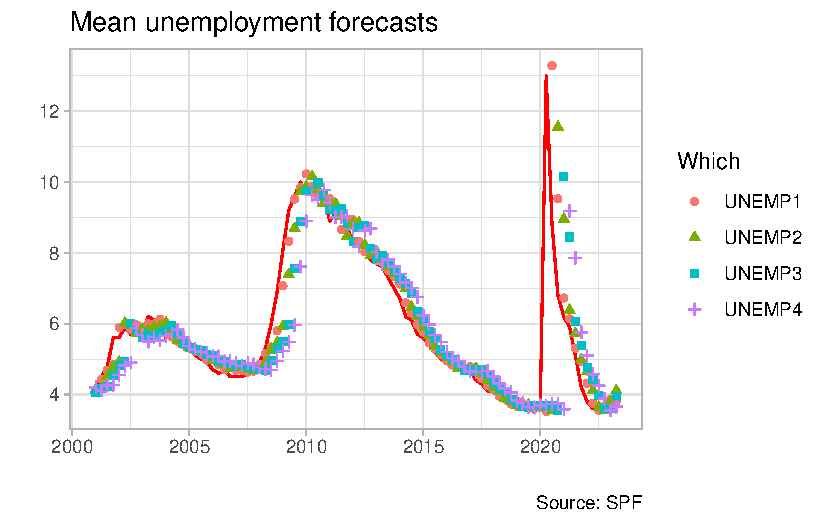
\includegraphics{./QR_files/figure-pdf/unnamed-chunk-2-1.pdf}

}

\end{figure}

\bookmarksetup{startatroot}

\hypertarget{causal-inference-in-statistics-pearl-glymour-jewell}{%
\chapter{Causal Inference in Statistics: Pearl, Glymour,
Jewell}\label{causal-inference-in-statistics-pearl-glymour-jewell}}

Outline how to solve the Pearl, Glymour, and Jewell (2016) exercises in
R.

\hypertarget{study-question-1.3.2}{%
\section{Study question 1.3.2}\label{study-question-1.3.2}}

Data:

\begin{Shaded}
\begin{Highlighting}[]
\FunctionTok{library}\NormalTok{(tidyverse)}
\NormalTok{ed }\OtherTok{\textless{}{-}} \FunctionTok{tibble}\NormalTok{(}\AttributeTok{Gender =} \FunctionTok{c}\NormalTok{(}\StringTok{"M"}\NormalTok{,}\StringTok{"M"}\NormalTok{,}\StringTok{"M"}\NormalTok{,}\StringTok{"M"}\NormalTok{,}\StringTok{"F"}\NormalTok{,}\StringTok{"F"}\NormalTok{,}\StringTok{"F"}\NormalTok{,}\StringTok{"F"}\NormalTok{),}
             \AttributeTok{eLevel =} \FunctionTok{c}\NormalTok{(}\StringTok{"U"}\NormalTok{,}\StringTok{"H"}\NormalTok{,}\StringTok{"C"}\NormalTok{,}\StringTok{"G"}\NormalTok{,}\StringTok{"U"}\NormalTok{,}\StringTok{"H"}\NormalTok{,}\StringTok{"C"}\NormalTok{,}\StringTok{"G"}\NormalTok{),}
             \AttributeTok{num    =} \FunctionTok{c}\NormalTok{(}\DecValTok{112}\NormalTok{,}\DecValTok{231}\NormalTok{,}\DecValTok{595}\NormalTok{,}\DecValTok{242}\NormalTok{,}\DecValTok{136}\NormalTok{,}\DecValTok{189}\NormalTok{,}\DecValTok{763}\NormalTok{,}\DecValTok{172}\NormalTok{)) }\SpecialCharTok{\%\textgreater{}\%}
  \FunctionTok{mutate}\NormalTok{(}\AttributeTok{total =} \FunctionTok{sum}\NormalTok{(num))}
\end{Highlighting}
\end{Shaded}

which we tabulate as

\begin{Shaded}
\begin{Highlighting}[]
\NormalTok{ed }\SpecialCharTok{\%\textgreater{}\%}
  \FunctionTok{kable}\NormalTok{()}
\end{Highlighting}
\end{Shaded}

\begin{longtable}[]{@{}llrr@{}}
\toprule()
Gender & eLevel & num & total \\
\midrule()
\endhead
M & U & 112 & 2440 \\
M & H & 231 & 2440 \\
M & C & 595 & 2440 \\
M & G & 242 & 2440 \\
F & U & 136 & 2440 \\
F & H & 189 & 2440 \\
F & C & 763 & 2440 \\
F & G & 172 & 2440 \\
\bottomrule()
\end{longtable}

\hypertarget{exercises-and-answers}{%
\section{Exercises and answers}\label{exercises-and-answers}}

\hypertarget{find-pelevel-h}{%
\subsection{\texorpdfstring{Find
\(P(eLevel = H)\)}{Find P(eLevel = H)}}\label{find-pelevel-h}}

\begin{Shaded}
\begin{Highlighting}[]
\NormalTok{ed }\SpecialCharTok{\%\textgreater{}\%}
  \FunctionTok{filter}\NormalTok{(eLevel }\SpecialCharTok{==} \StringTok{"H"}\NormalTok{) }\SpecialCharTok{\%\textgreater{}\%}
  \FunctionTok{mutate}\NormalTok{(}\AttributeTok{p\_H =} \FunctionTok{sum}\NormalTok{(num)}\SpecialCharTok{/}\NormalTok{total) }\SpecialCharTok{\%\textgreater{}\%}
  \FunctionTok{kable}\NormalTok{()}
\end{Highlighting}
\end{Shaded}

\begin{longtable}[]{@{}llrrr@{}}
\toprule()
Gender & eLevel & num & total & p\_H \\
\midrule()
\endhead
M & H & 231 & 2440 & 0.1721311 \\
F & H & 189 & 2440 & 0.1721311 \\
\bottomrule()
\end{longtable}

\hypertarget{find-pelevel-h-vee-gender-f}{%
\subsection{\texorpdfstring{Find
\(P(eLevel = H\ \vee \ Gender = F)\)}{Find P(eLevel = H\textbackslash{} \textbackslash vee \textbackslash{} Gender = F)}}\label{find-pelevel-h-vee-gender-f}}

\begin{Shaded}
\begin{Highlighting}[]
\NormalTok{ed }\SpecialCharTok{\%\textgreater{}\%}
  \FunctionTok{filter}\NormalTok{(Gender }\SpecialCharTok{==} \StringTok{"F"} \SpecialCharTok{|}\NormalTok{ eLevel }\SpecialCharTok{==} \StringTok{"H"}\NormalTok{) }\SpecialCharTok{\%\textgreater{}\%}
  \FunctionTok{mutate}\NormalTok{(}\AttributeTok{p\_HorF =} \FunctionTok{sum}\NormalTok{(num)}\SpecialCharTok{/}\NormalTok{total) }\SpecialCharTok{\%\textgreater{}\%}
  \FunctionTok{kable}\NormalTok{()}
\end{Highlighting}
\end{Shaded}

\begin{longtable}[]{@{}llrrr@{}}
\toprule()
Gender & eLevel & num & total & p\_HorF \\
\midrule()
\endhead
M & H & 231 & 2440 & 0.6110656 \\
F & U & 136 & 2440 & 0.6110656 \\
F & H & 189 & 2440 & 0.6110656 \\
F & C & 763 & 2440 & 0.6110656 \\
F & G & 172 & 2440 & 0.6110656 \\
\bottomrule()
\end{longtable}

\hypertarget{find-pelevel-h-gender-f}{%
\subsection{\texorpdfstring{Find
\(P(eLevel = H\ |\ Gender = F)\)}{Find P(eLevel = H\textbackslash{} \textbar\textbackslash{} Gender = F)}}\label{find-pelevel-h-gender-f}}

\begin{Shaded}
\begin{Highlighting}[]
\NormalTok{ed }\SpecialCharTok{\%\textgreater{}\%}
  \FunctionTok{filter}\NormalTok{(Gender }\SpecialCharTok{==} \StringTok{"F"}\NormalTok{) }\SpecialCharTok{\%\textgreater{}\%}
  \FunctionTok{mutate}\NormalTok{(}\AttributeTok{tcond =} \FunctionTok{sum}\NormalTok{(num)) }\SpecialCharTok{\%\textgreater{}\%} 
  \FunctionTok{filter}\NormalTok{(eLevel }\SpecialCharTok{==} \StringTok{"H"}\NormalTok{) }\SpecialCharTok{\%\textgreater{}\%}
  \FunctionTok{mutate}\NormalTok{(}\AttributeTok{p\_HgivenF =} \FunctionTok{sum}\NormalTok{(num)}\SpecialCharTok{/}\NormalTok{tcond) }\SpecialCharTok{\%\textgreater{}\%}
  \FunctionTok{kable}\NormalTok{()}
\end{Highlighting}
\end{Shaded}

\begin{longtable}[]{@{}llrrrr@{}}
\toprule()
Gender & eLevel & num & total & tcond & p\_HgivenF \\
\midrule()
\endhead
F & H & 189 & 2440 & 1260 & 0.15 \\
\bottomrule()
\end{longtable}

\hypertarget{find-pgender-f-elevel-h}{%
\subsection{\texorpdfstring{Find
\(P(Gender = F\ | \ eLevel = H)\)}{Find P(Gender = F\textbackslash{} \textbar{} \textbackslash{} eLevel = H)}}\label{find-pgender-f-elevel-h}}

\begin{Shaded}
\begin{Highlighting}[]
\NormalTok{ed }\SpecialCharTok{\%\textgreater{}\%}
  \FunctionTok{filter}\NormalTok{(eLevel }\SpecialCharTok{==} \StringTok{"H"}\NormalTok{) }\SpecialCharTok{\%\textgreater{}\%}
  \FunctionTok{mutate}\NormalTok{(}\AttributeTok{tcond =} \FunctionTok{sum}\NormalTok{(num)) }\SpecialCharTok{\%\textgreater{}\%} 
  \FunctionTok{filter}\NormalTok{(Gender }\SpecialCharTok{==} \StringTok{"F"}\NormalTok{) }\SpecialCharTok{\%\textgreater{}\%}
  \FunctionTok{mutate}\NormalTok{(}\AttributeTok{p\_FgivenH =} \FunctionTok{sum}\NormalTok{(num)}\SpecialCharTok{/}\NormalTok{tcond) }\SpecialCharTok{\%\textgreater{}\%}
  \FunctionTok{kable}\NormalTok{()}
\end{Highlighting}
\end{Shaded}

\begin{longtable}[]{@{}llrrrr@{}}
\toprule()
Gender & eLevel & num & total & tcond & p\_FgivenH \\
\midrule()
\endhead
F & H & 189 & 2440 & 420 & 0.45 \\
\bottomrule()
\end{longtable}

\bookmarksetup{startatroot}

\hypertarget{summary}{%
\chapter{Summary}\label{summary}}

In summary, this book has no content whatsoever\ldots{}

\bookmarksetup{startatroot}

\hypertarget{references}{%
\chapter*{References}\label{references}}
\addcontentsline{toc}{chapter}{References}

\markboth{References}{References}

\hypertarget{refs}{}
\begin{CSLReferences}{1}{0}
\leavevmode\vadjust pre{\hypertarget{ref-Mumtaz_BOOK}{}}%
Blake, Andrew P, and Haroon Mumtaz. 2017. \emph{Applied Bayesian
Econometrics for Central Bankers}. Revised. Technical Books. Centre for
Central Banking Studies, Bank of England.

\leavevmode\vadjust pre{\hypertarget{ref-HOMLR}{}}%
Boehmke, Brad, and Brandon M. Greenwell. 2019. \emph{Hands-on Machine
Learning with {R}}. The {R} Series. Boca Raton: Chapman \& Hall/CRC.
\url{https://bradleyboehmke.github.io/HOML/}.

\leavevmode\vadjust pre{\hypertarget{ref-Mixtape}{}}%
Cunningham, Scott. 2021. \emph{Causal Inference: The Mixtape}. New Haven
\& London: Yale University Press. \url{https://mixtape.scunning.com/}.

\leavevmode\vadjust pre{\hypertarget{ref-GHV}{}}%
Gelman, Andrew, Jennifer Hill, and Aki Vehtari. 2019. \emph{Regression
and Other Stories}. Cambridge: Cambridge University Press.
\url{http://www.stat.columbia.edu/~gelman/regression}.

\leavevmode\vadjust pre{\hypertarget{ref-ESL}{}}%
Hastie, Trevor, Robert Tibshirani, and Jerome Friedman. 2009. \emph{The
Elements of Statistical Learning: Data Mining, Inference, and
Prediction}. 2nd ed. New York, NY: Springer.
\url{https://web.stanford.edu/~hastie/ElemStatLearn/}.

\leavevmode\vadjust pre{\hypertarget{ref-SuperText}{}}%
Hvitfeldt, Emil, and Julia Silge. 2021. \emph{Supervised Machine
Learning for Text Analysis in {R}}. Chapman \& Hall: CRC Press.
\url{https://smltar.com/}.

\leavevmode\vadjust pre{\hypertarget{ref-ITSL}{}}%
James, Gareth, Daniela Witten, Trevor Hastie, and Robert Tibshirani.
2021. \emph{An Introduction to Statistical Learning: With Applications
in {R}}. 2nd ed. Springer Texts in Statistics. New York, NY: Springer.
\url{https://www.statlearning.com/}.

\leavevmode\vadjust pre{\hypertarget{ref-Geocomputation}{}}%
Lovelace, Robin, Jakub Nowosad, and Jannes Muenchow. 2019.
\emph{Geocomputation with {R}}. 1st ed. The {R} Series. Boca Raton:
Chapman \& Hall/CRC. \url{https://geocompr.robinlovelace.net/}.

\leavevmode\vadjust pre{\hypertarget{ref-McElreath}{}}%
McElreath, Richard. 2020. \emph{Statistical Rethinking: A Bayesian
Course with Examples in {R} and Stan}. 2nd ed. Abingdon, Oxfordshire:
CRC Press. \url{https://github.com/rmcelreath/rethinking}.

\leavevmode\vadjust pre{\hypertarget{ref-Primer}{}}%
Pearl, Judea, Madelyn Glymour, and Nicholas P. Jewell. 2016.
\emph{Causal Inference in Statistics: A Primer}. Chichester: John Wiley
\& Sons. \url{http://bayes.cs.ucla.edu/PRIMER/}.

\leavevmode\vadjust pre{\hypertarget{ref-Silge}{}}%
Silge, Julia, and David Robinson. 2017. \emph{Text Mining with {R}: A
{T}idy Approach}. O'Reilly. \url{https://www.tidytextmining.com/}.

\leavevmode\vadjust pre{\hypertarget{ref-Taddy}{}}%
Taddy, Matt. 2019. \emph{Business Data Science: Combining Machine
Learning and Economics to Optimize, Automate, and Accelerate Business
Decisions}. New York, NY: McGraw-Hill Education.
\url{https://github.com/TaddyLab/BDS}.

\end{CSLReferences}


\backmatter

\end{document}
